\documentclass[11pt]{article}
\usepackage[T1]{fontenc}
\usepackage[utf8]{inputenc}
\usepackage[spanish]{babel}
\usepackage{amsmath, amssymb}
\usepackage{graphicx}
\usepackage{hyperref}
\usepackage{geometry}
\usepackage{fancyhdr}
\usepackage{listings}
\usepackage{xcolor}
\geometry{a4paper, margin=2.5cm}

\lstdefinestyle{mystyle}{
backgroundcolor=\color{gray!10},
commentstyle=\color{green!50!black},
keywordstyle=\color{blue},
numberstyle=\tiny\color{gray},
stringstyle=\color{red!70!brown},
basicstyle=\ttfamily\small,
breaklines=true,
captionpos=b,
keepspaces=true,
numbers=left,
numbersep=5pt,
showspaces=false,
showstringspaces=false,
showtabs=false,
frame=single,
language=Matlab
}

\lstset{style=mystyle}

\title{\Huge Sistemas de Control II\\[0.4cm] \Large Tarea 4: Estabilización de un Péndulo Simple con Acción Integral}
\date{}

\begin{document}

% Carátula
%\centering
\begin{centering}
\vspace*{2cm}
{\Huge\bfseries Sistemas de Control II \par}
\vspace{0.5cm}
{\Large Tarea 3: Estabilización de un Péndulo Simple \par}
\vspace{2cm}
\large
\textbf{Profesor:} Sergio Laboret\\[0.3cm]

\textbf{Alumno:} Angeloff Jorge

\end{centering}
\newpage
\section*{1. Modelado del sistema no lineal}

Se parte de la ecuación del péndulo simple:
\begin{equation}
ml^2 \ddot{\theta} + b \dot{\theta} + mgl \sin(\theta) = T
\end{equation}

El objetivo es estabilizar el péndulo en un ángulo $\delta$. Se define el error como $e(t) = \delta - \theta(t)$.

La entrada es el torque aplicado $T$, y la salida es $\theta$.

\subsection*{Código MATLAB}
\begin{lstlisting}
m = 2;
b = 0.3;
l = 1;
G = 10;
delta = 135;
\end{lstlisting}

\subsection*{Sistema en variables de estado}

Se definen los estados como:

\[
x_1 = \theta - \delta, \quad x_2 = \dot{\theta}
\]

Entonces, el sistema dinámico en coordenadas desplazadas (alrededor del punto de equilibrio deseado) se escribe como:

\[
\dot{x}_1 = x_2
\]
\[
\dot{x}_2 = \frac{1}{ml^2} \left( -b x_2 - mgl \sin(x_1 + \delta) + T \right)
\]

Por lo tanto:

\[
\dot{x} = f(x,u) = 
\begin{bmatrix}
x_2 \\
\frac{1}{ml^2} \left( -b x_2 - mgl \sin(x_1 + \delta) + u \right)
\end{bmatrix},
\quad
y = h(x) = x_1
\]



\section*{2. Linealización y torque de equilibrio}
Para hallar el torque necesario que equilibra el sistema en $\theta = \delta$, se impone $\ddot{\theta} = \dot{\theta} = 0$, por lo tanto:
\begin{equation}
    u_f = mgl \sin(\delta)
\end{equation}

Luego se linealiza el sistema no lineal alrededor del punto de equilibrio $\theta = \delta$, resultando un modelo lineal en coordenadas locales.

\subsection*{Código MATLAB}
\begin{lstlisting}
[A,B,C,D] = linmod('pendulo_mod_tarea', delta*pi/180);
eig(A)
rank(ctrb(A,B))
\end{lstlisting}


Los parámetros del sistema son: \( m = 2 \,\mathrm{kg},\ l = 1 \,\mathrm{m},\ b = 0{,}3 \,\mathrm{N\,m\,s},\ \delta = 135^\circ \).

El torque de equilibrio se calcula como:
\[
    u_f = mgl \sin(\delta) = 2 \cdot 9{,}81 \cdot 1 \cdot \sin(135^\circ) \approx 13{,}87 \,\mathrm{Nm}
\]

La linealización dio como resultado la siguiente representación en espacio de estados:

\[
A = \begin{bmatrix}
0 & 1 \\
7{,}0711 & -0{,}1500
\end{bmatrix}, \quad
B = \begin{bmatrix}
0 \\
0{,}5
\end{bmatrix}, \quad
C = \begin{bmatrix}
1 & 0
\end{bmatrix}, \quad
D = 0
\]

Los autovalores del sistema linealizado son:
\[
\lambda_1 = 2{,}5852, \quad \lambda_2 = -2{,}7352
\]

Ambos son reales y de signo opuesto, lo cual confirma que el punto de equilibrio linealizado es un punto de silla, es decir, inestable.


Además, la matriz de controlabilidad tiene rango completo:
\[
\text{rango}(\mathcal{C}) = 2
\]
por lo tanto, el sistema linealizado es completamente controlable.

\section*{3. Controlador con acción integral}
Para asegurar el seguimiento de referencia sin error en régimen permanente, se incorpora una acción integral al sistema. Se define una nueva variable de estado:
\[
\sigma(t) = \int_0^t (r(\tau) - y(\tau)) \, d\tau
\]
donde \( r(t) \) es la referencia y \( y(t) \) la salida del sistema. En este caso, \( r = \delta \) y \( y = x_1 = \theta - \delta \), por lo que la señal de error es simplemente \( -x_1 \).

El vector de estados extendido es:
\[
x_a = \begin{bmatrix} x_1 \\ x_2 \\ \sigma \end{bmatrix}
\]

Y la ley de control se plantea como:
\[
u = -Kx - k_i \sigma = -[k_1 \quad k_2 \quad k_3] \begin{bmatrix} x_1 \\ x_2 \\ \sigma \end{bmatrix}
\]

\subsection*{Código MATLAB}
\begin{lstlisting}
Aa = [[A; C], zeros(3,1)];
Ba = [B; 0];
eig(Aa)
rank(ctrb(Aa, Ba))
K = acker(Aa, Ba, [p p p]);
k1 = K(1);
k2 = K(2);
k3 = K(3);
eig(Aa - Ba * K)
tscalc = 7.5 / (-p);
\end{lstlisting}


La matriz del sistema extendido y el vector de entrada quedan definidos como:
\[
A_a = \begin{bmatrix}
0 & 1 & 0 \\
7{,}0711 & -0{,}15 & 0 \\
1 & 0 & 0
\end{bmatrix}, \quad
B_a = \begin{bmatrix}
0 \\ 0{,}5 \\ 0
\end{bmatrix}
\]

Los autovalores del sistema extendido sin control son:
\[
\lambda = \{0,\ -2{,}7352,\ 2{,}5852\}
\]
Por lo tanto el sistema es inestable pero controlable, como ya se vio, lo cual permite diseñar un controlador por asignación de polos.

Se eligieron polos deseados en \( s = -4 \) (polo triple), y se obtuvo:
\[
K = [k_1 \quad k_2 \quad k_3] = [110{,}14 \quad 23{,}70 \quad 128]
\]

Los autovalores del sistema cerrado resultaron:
\[
\lambda_{\text{LC}} = \{-4,\ -4,\ -4\}
\]
y el tiempo de establecimiento estimado con la fórmula \( t_s = \frac{7{,}5}{|\text{Re}(p)|} \) es:
\[
t_s \approx 1{,}875 \text{ s}
\]

Esto asegura una respuesta rápida y estable, con rechazo de error estacionario frente a cambios de referencia o perturbaciones constantes.

\section*{4. Simulación en Simulink y resultados}
\subsection*{Código MATLAB}
\begin{lstlisting}
sim('pendulo_pid_tarea')
figure(1), plot(tout, yout)
figure(2), plot(yout, velocidad)
figure(3), plot(tout, torque)
figure(4), plot(tout, -accint)
ymax = max(yout);
S = (ymax - delta) / delta * 100;
erel = (delta - yout) / delta;
ef = erel(end);
ind = find(abs(erel) > 0.02);
tss = tout(ind(end));
yte = yout(ind(end));
uf = torque(end);
Intf = -accint(end);
\end{lstlisting}

\subsection*{Análisis de resultados}

Se simula el sistema con el controlador diseñado para estabilizar el péndulo en el ángulo de referencia \( \delta = 135^\circ \). Los principales resultados obtenidos son:

\begin{itemize}
  \item \textbf{Sobrepaso:} \( y_{\text{máx}} = 160{,}52^\circ \Rightarrow S = 18{,}9\% \)
  \item \textbf{Error en régimen permanente:} \( e_{\infty} \approx 2{,}88 \times 10^{-14} \Rightarrow \textbf{ess} = 0 \)
  \item \textbf{Tiempo de establecimiento (2\%):} \( t_s = 1{,}804 \ \text{s} \)
  \item \textbf{Valor final del torque aplicado:} \( u_f = 14{,}14 \)
  \item \textbf{Valor final de la acción integral:} \( \sigma_{\text{final}} = 14{,}14 \)
\end{itemize}

Estos resultados confirman que el sistema alcanza rápidamente el régimen estacionario con error cero, como se esperaba por la inclusión de la acción integral. El sobrepaso observado es moderado y aceptable para esta aplicación.
\newpage

\subsection*{Descripción de las figuras}


    \begin{figure}[ht]
          \centering
            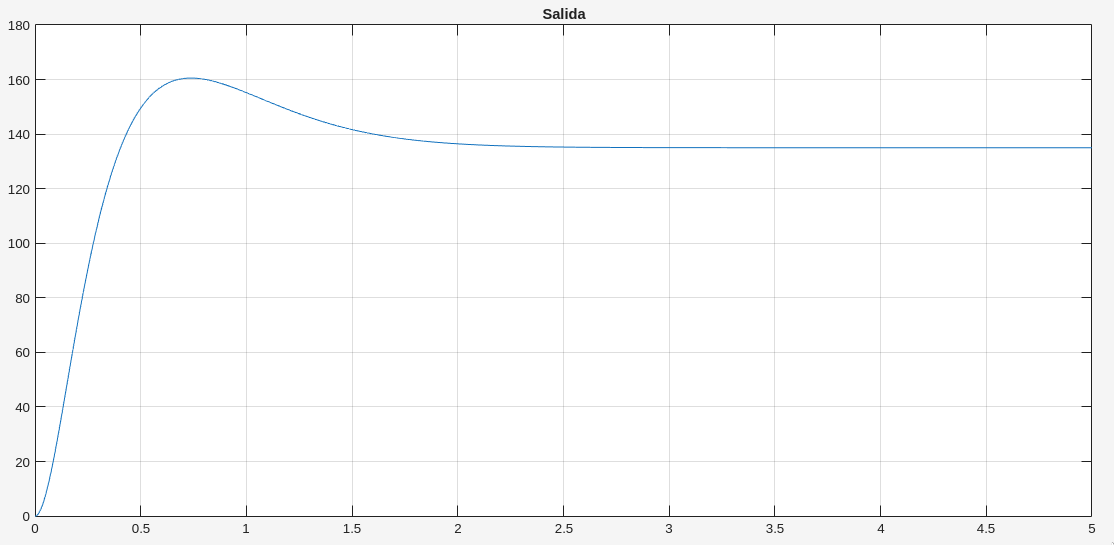
\includegraphics[width=1\textwidth]{/home/jorge/Documentos/FCEFyN/SC2/SC2_2025/l_tarea_3/informe/capturas/figure1.png}
              \caption{Respuesta del sistema.}
            \end{figure} 

\textbf{Figura 1: Respuesta del sistema.} Se observa que la salida parte desde 0 y alcanza el valor deseado de \( 135^\circ \), con un sobrepaso hasta \( 160{,}52^\circ \) a los \( 0{,}735 \ \text{s} \). El error cae por debajo del 2\% antes de los \( 1{,}8 \ \text{s} \).


    \begin{figure}[ht]
          \centering
            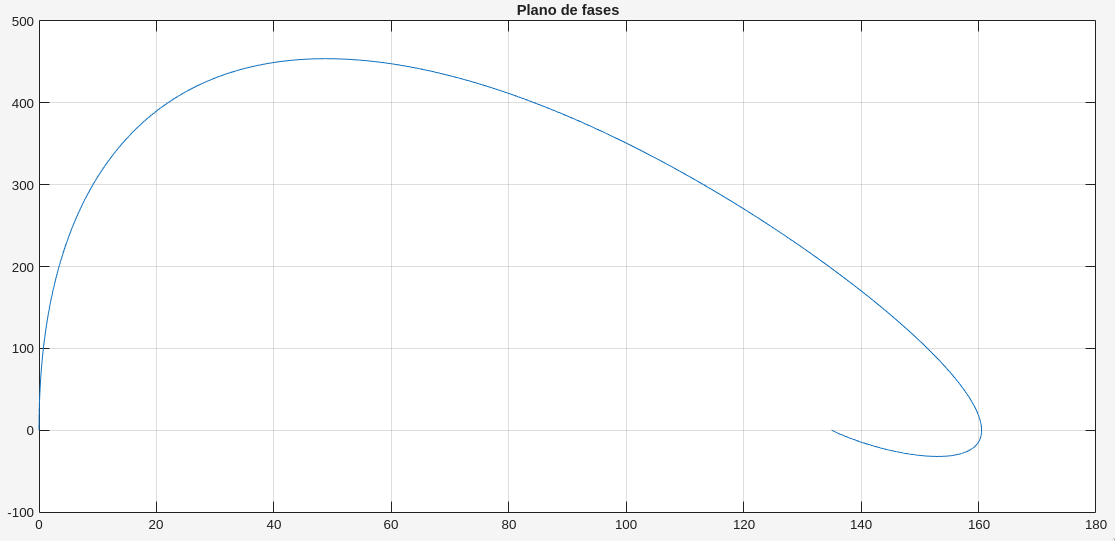
\includegraphics[width=1\textwidth]{/home/jorge/Documentos/FCEFyN/SC2/SC2_2025/l_tarea_3/informe/capturas/figure2.png}
              \caption{Plano de fases.}
            \end{figure} 

\textbf{Figura 2: Plano de fases.} Se representa la evolución del sistema en el espacio de estados \((x_1, x_2) = (\theta - \delta, \dot{\theta})\). El sistema describe una espiral hacia adentro, lo que indica una trayectoria típicamente subamortiguada pero estable, convergiendo al punto de equilibrio.


    \begin{figure}[ht]
          \centering
            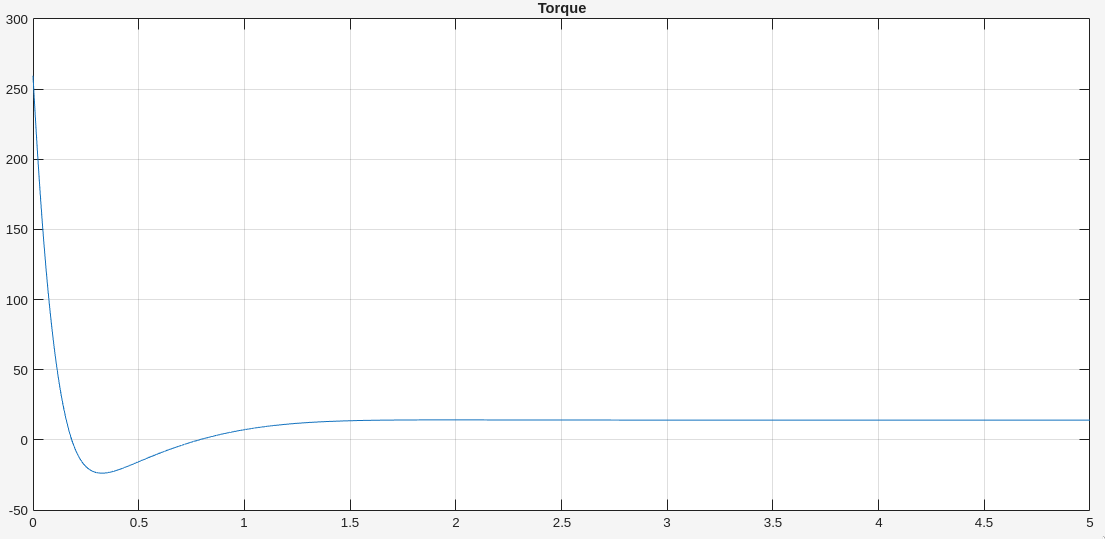
\includegraphics[width=1\textwidth]{/home/jorge/Documentos/FCEFyN/SC2/SC2_2025/l_tarea_3/informe/capturas/figure3.png}
              \caption{Torque aplicado.}
            \end{figure} 
\newpage

\textbf{Figura 3: Torque aplicado.} El torque arranca desde un valor alto (\( \sim 259{,}5 \,Nm \)), luego presenta un mínimo negativo de \( -25{,}18 \, Nm \) a los \( 0{,}35 \ \text{s} \), y finalmente se estabiliza en \( 15{,}55 \, Nm \), muy cerca del valor de equilibrio teórico calculado \( u_f = mgl \sin(\delta)=13.87 \, Nm \).

    \begin{figure}[ht]
          \centering
            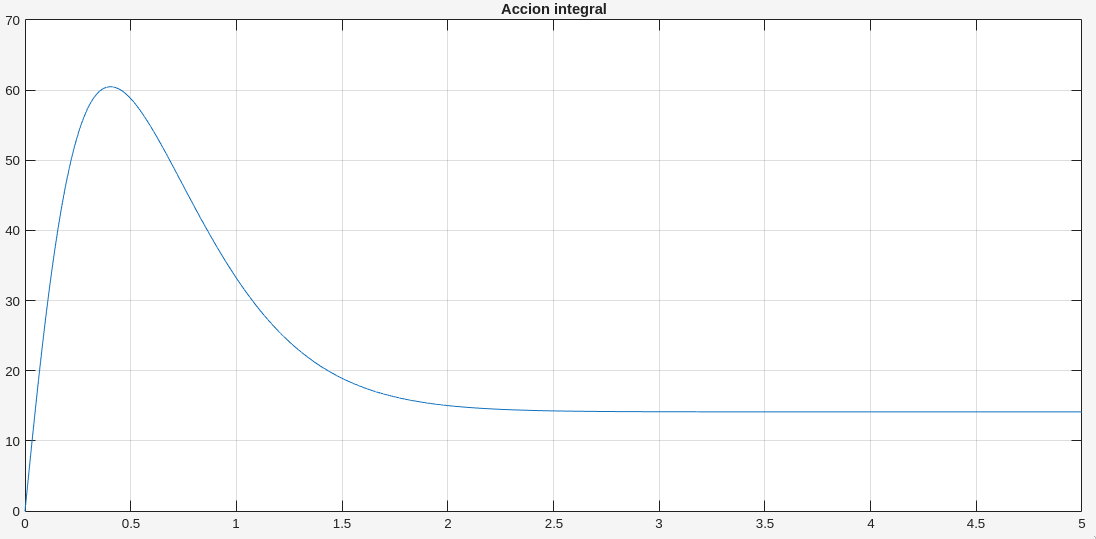
\includegraphics[width=1\textwidth]{/home/jorge/Documentos/FCEFyN/SC2/SC2_2025/l_tarea_3/informe/capturas/figure4.png}
              \caption{Acción integral.}
            \end{figure} 

\textbf{Figura 4: Acción integral.} Muestra un sobrepico de \( 61{,}87 \) a los \( 0{,}41 \ \text{s} \), para luego estabilizarse en \( 15{,}55 \). Esto refleja cómo la acción integral acumula el error inicial y contribuye a corregirlo, asegurando el rechazo total del error en régimen.


\section*{5. Análisis de robustez}
Se evalúa la robustez del controlador frente a variaciones en la masa \( m \). Se analiza cómo afectan al sobrepaso, el tiempo de establecimiento, el valor final del torque y la acción integral. En particular, se prueba el sistema con masas del 90\%, 100\% y 110\% de la nominal.

\subsection*{Código MATLAB}
\begin{lstlisting}
m_nom = 2;
variaciones_masa = [0.9, 1.0, 1.1];
resultados = zeros(3, 4);

for i = 1:3
    m = variaciones_masa(i) * m_nom;
    sim('pendulo_pid_tarea');
    ymax = max(yout);
    S = (ymax - delta)/delta * 100;
    erel = (delta - yout)/delta;
    ind = find(abs(erel) > 0.02);
    tss = tout(ind(end));
    uf = torque(end);
    Intf = -accint(end);
    resultados(i,:) = [S, tss, uf, Intf];
end
\end{lstlisting}

\subsection*{Tabla de resultados}
\begin{center}
\begin{tabular}{|c|c|c|c|c|}
\hline
\textbf{Masa} & \textbf{Sobrepaso (\%)} & \textbf{\(T_s\) (s)} & \textbf{\(u_f\)} & \textbf{\(\sigma\) final} \\
\hline
1.8 m & 17.90 & 1.87 & 12.73 & 12.73 \\
2.0 m & 18.91 & 1.80 & 14.14 & 14.14 \\
2.2 m & 20.01 & 1.73 & 15.56 & 15.56 \\
\hline
\end{tabular}
\end{center}

\subsection*{Análisis}

Se observa que:

\begin{itemize}
  \item El \textbf{tiempo de establecimiento} disminuye levemente al aumentar la masa. Esto es esperable ya que el torque requerido para estabilizar es mayor, lo que provoca una respuesta más enérgica.
  \item El \textbf{sobrepaso} se incrementa con la masa, aunque dentro de un rango aceptable, lo que indica que el controlador mantiene buen desempeño a pesar de la variación.
  \item El \textbf{valor final del torque} y de la \textbf{acción integral} crecen proporcionalmente con la masa, lo que refleja correctamente la relación \( u_f = mgl \sin(\delta) \). Esto demuestra que la acción integral compensa adecuadamente la variación de carga estática.
\end{itemize}

\newpage

\subsection*{Graficos}

 \begin{figure}[ht]
          \centering
            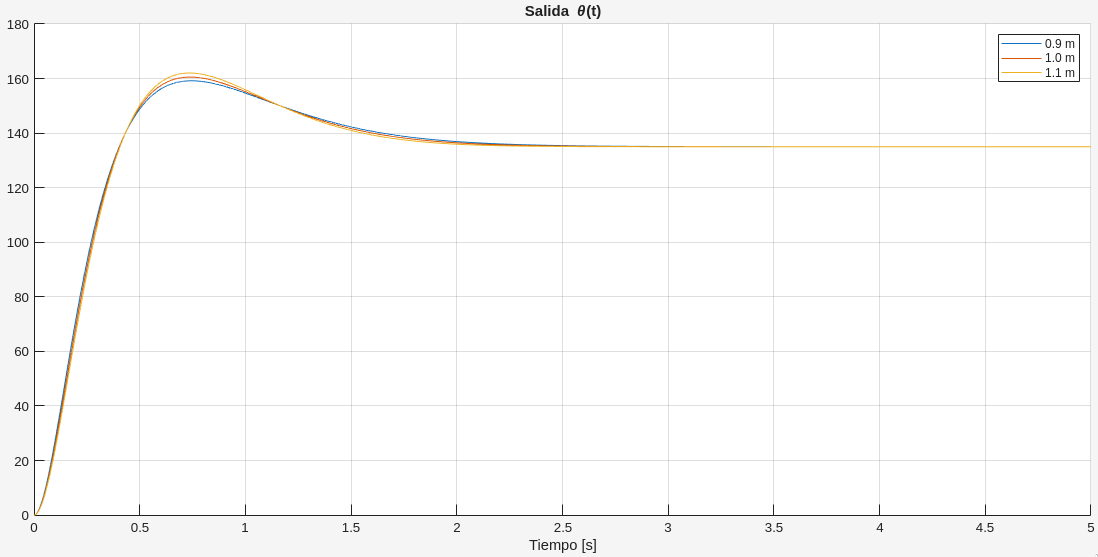
\includegraphics[width=1\textwidth]{/home/jorge/Documentos/FCEFyN/SC2/SC2_2025/l_tarea_3/informe/capturas/f1.png}
              \caption{Respuesta del sistema.}
            \end{figure} 


    \begin{figure}[ht]
          \centering
            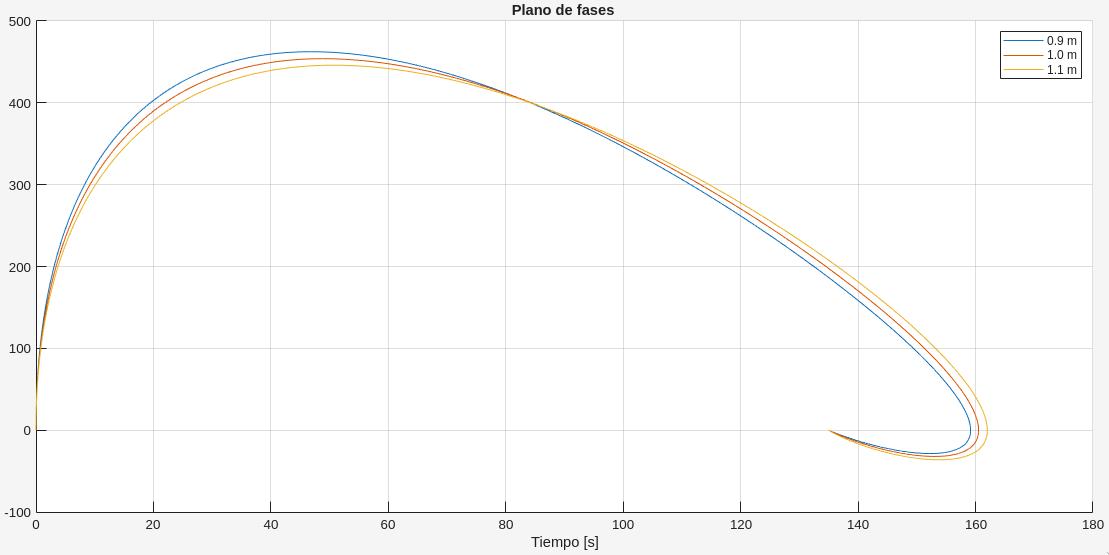
\includegraphics[width=1\textwidth]{/home/jorge/Documentos/FCEFyN/SC2/SC2_2025/l_tarea_3/informe/capturas/f2.png}
              \caption{Plano de fases.}
            \end{figure} 
\newpage

    \begin{figure}[ht]
          \centering
            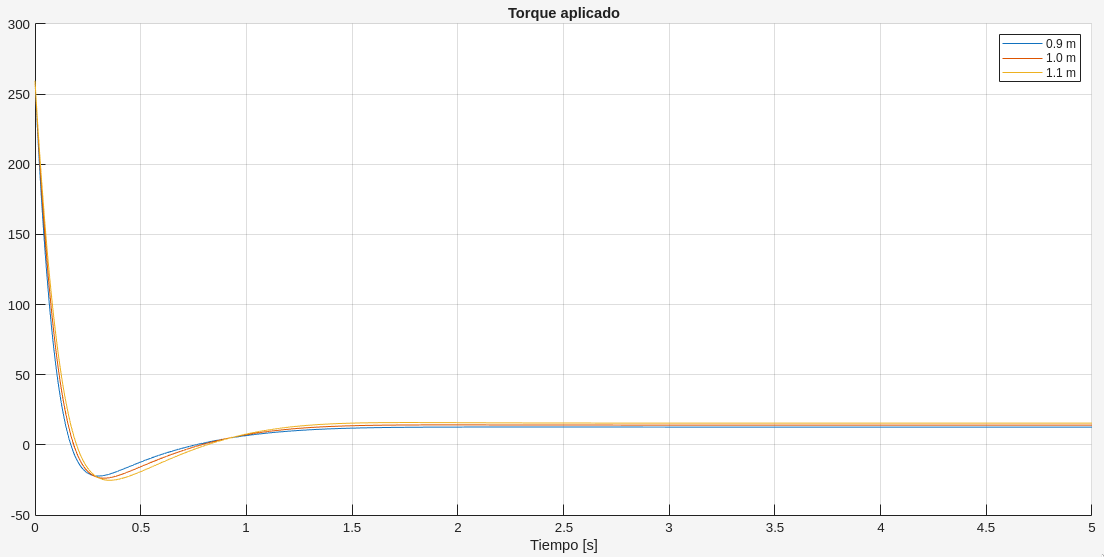
\includegraphics[width=1\textwidth]{/home/jorge/Documentos/FCEFyN/SC2/SC2_2025/l_tarea_3/informe/capturas/f3.png}
              \caption{Torque aplicado.}
            \end{figure} 


    \begin{figure}[ht]
          \centering
            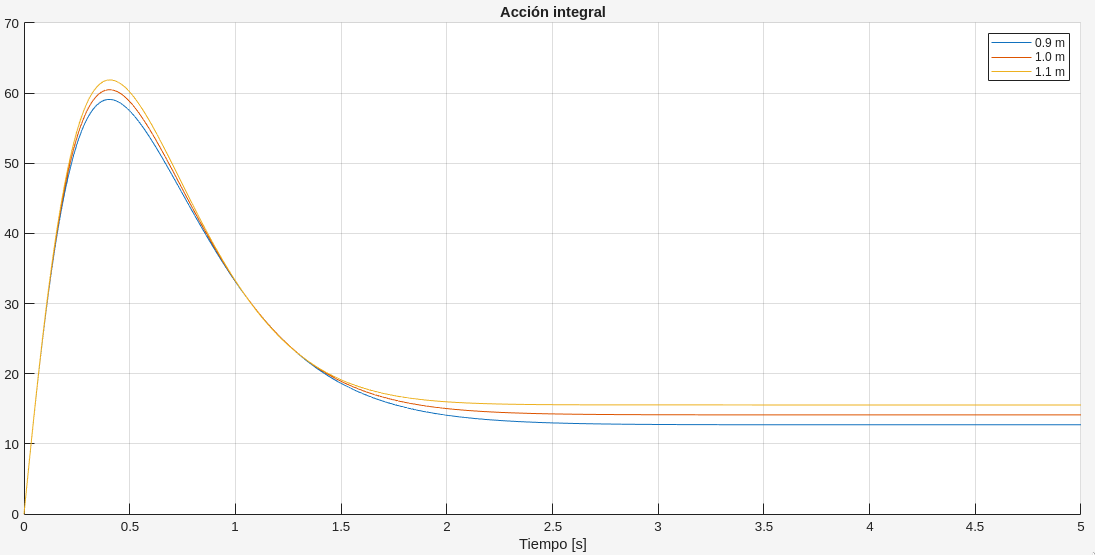
\includegraphics[width=1\textwidth]{/home/jorge/Documentos/FCEFyN/SC2/SC2_2025/l_tarea_3/informe/capturas/f4.png}
              \caption{Acción integral.}
            \end{figure} 


En conjunto, los resultados muestran que el sistema controlado es robusto frente a variaciones moderadas de masa.

\section*{6. Conclusiones}

En esta tarea se diseñó y analizó un controlador con acción integral para estabilizar un péndulo simple en un ángulo arbitrario. A partir de la linealización del modelo no lineal, se aplicó asignación de polos sobre el sistema extendido, garantizando estabilidad y seguimiento exacto de la referencia.

Las simulaciones mostraron buen desempeño dinámico: tiempo de establecimiento menor a 2 segundos, sobrepaso moderado ($\approx 19\%$) y error estacionario nulo. La acción integral fue clave para alcanzar el equilibrio deseado.

Además, se evaluó la robustez ante variaciones del $10\%$ en la masa, observando un comportamiento estable con cambios leves en la dinámica. Esto confirma que el controlador es robusto frente a perturbaciones en la carga.

En resumen, el controlador cumple con los objetivos de estabilidad, seguimiento y robustez frente a variaciones paramétricas.

\end{document}

